\documentclass[spanish]{article}
\usepackage{graphicx}
\usepackage{ragged2e}
\usepackage{geometry}
\usepackage{float}
\usepackage{hyperref}
\usepackage[table,xcdraw]{xcolor}
\usepackage[ruled,vlined]{algorithm2e}
\title {Práctica 5: Algoritmos Greedy}
\graphicspath{{../img/}}
\addtolength{\textheight}{1.5in} 
\begin{document}
	\centerline{
\includegraphics[width=450px,height=100px]{header}}
	\centerline{Analisis de algoritmos, Sem: 2021-1, 3CV1,Práctica  3, 11/11/2020}
	\centering{\huge{Práctica 5: Algoritmos Greedy}}
	\centerline{\newline{\textbf{Payán Téllez René}}}
	\newline{\textit{rpayant1500@alumno.ipn.mx}}
	\bigskip
	\justify
	\textbf{Resumen:}	
	En esta practica se analizaran 2 algoritmos que utilizan la tecnica de divide y venceras para resolver un problema, uno de ellos el quick sort y otro el sub arreglo maximo.\\
	\textbf{Palabras clave:}
	QuickSort,SubArreglo maximo,divide y venceras,C/C++
	\section{Introduccion}
	
	\section{Conceptos Basicos}
	\subsection{Algoritmo}
		La palabra algoritmo proviene del sobrenombre de un matemático árabe del siglo IX, Al-Khwarizmi, que fue reconocido por enunciar paso a paso las reglas para las operaciones matemáticas básicas con decimales (suma, resta, multiplicación y división).	
		Vemos definición de algoritmo como un grupo de órdenes consecutivas que presentan una solución a un problema o tarea. Algunos ejemplos de algoritmos los podemos encontrar en las matemáticas (como el algoritmo para resolver una multiplicación) y en los manuales de usuario de un aparato (como una lavadora o una impresora).	
		Sin embargo, hoy en día se relaciona la palabra algoritmo con el mundo de la informática, más concretamente en la programación; los conocidos como algoritmos informáticos.[1]
	\subsection{Complejidad algoritmica}
		Así que, por su naturaleza, un problema tiene la capacidad de ser solucionado por uno o varios métodos, pero si bien es importante llegar a la respuesta, más importante es evaluar su viabilidad. Siempre que se analiza y evalúa adecuadamente la efectividad de una solución, disminuye drásticamente el costo que representa su producción y mantenimiento, pues los recursos que se invierten posteriormente en codificación, pruebas y revisión es mucho menor siempre (como el tiempo, dinero y talento humano).	
		Entrando en materia, la complejidad algorítmica es una métrica teórica que nos ayuda a describir el comportamiento de un algoritmo en términos de tiempo de ejecución (tiempo que tarda un algoritmo en resolver un problema) y memoria requerida (cantidad de memoria necesaria para procesar las instrucciones que solucionan dicho problema). Esto nos ayuda a comparar entre la efectividad de un algoritmo y otro, y decidir cuál es el que nos conviene implementar.[2]
	\subsection{Algoritmos Greedy o glotones}	
		Un algoritmo Greedy o gloton es un algoritmo muy util para encontrar soluciones aproximadas e inclusive la mas optima a problemas complejos, ya que las entregan en muy corto tiempo. Se llaman Greedy porque siempre "comen lo que tienen a la mano", no garantizan encontrar la mejor solucion, pero si una aproximacion bastante buena.[3]
		Estas son sus caracteristicas principales:
		\begin{itemize}
			\item Se utilizan generalmente para resolver problemas deoptimización (obtener el máximo o el mínimo).optimización (obtener el máximo o el mínimo).
			\item Toman decisiones en función de la información que está disponible en cada momento. está disponible en cada momento. está disponible en cada momento. está disponible en cada momen
			\item Una vez tomada la decisión, ésta no vuelve a replantearse en el futuro.replantearse en el futuro.
			\item Suelen ser rápidos y fáciles de implementar.
			\item No siempre garantizan alcanzar la solución óptima[4]
		\end{itemize}
	\subsection{Algoritmo de codificación de Huffman}
		El código de Huffman es un tipo particular de código de prefijo óptimo que se usa comúnmente para la compresión de datos sin pérdida. Comprime los datos de manera muy efectiva, ahorrando de 20$\%$ a 90$\%$ de memoria, dependiendo de las características de los datos comprimidos. Este algoritmo se aplica solo si se considera a la entrada como una cadena de caracteres, ya que es un algoritmo boraz que utiliza una tabla que proporciona la frecuencia con la que aparece cada carácter (es decir, su frecuencia) para crear una forma óptima de representar cada carácter como una cadena binaria. Fue propuesto por David A. Huffman en 1951.[5]
		\begin{algorithm}[H]
			\KwData{Entrada: C(Cadena a codificar)}
			\KwResult{Retorna }
			x=A[r]\;
			i=p-1\;
			\For{$j\gets p$ \KwTo $j \leq r-1$}{
				\If{$A[j] \leq x$}{
					i++\;
					exchange(A[i],A[j]);
				}
			}
			exchange(A[i+1],A[r])\;
			return i+1\;
			\caption{Partition A[p,...,r]}
		\end{algorithm}
	\begin{algorithm}[H]
		\KwData{Entrada: A[p,...,n]}
		\KwResult{Retorna un areglo ordenado de forma ascendente}
		\If{$p < n$}{
			q=Partition(A,p,n)\;
			QuickSort(A,p,q-1)\;
			QuickSort(A,q+1,n)\;
		}
		\caption{QuickSort A[p,...,n]}
	\end{algorithm}
	\subsection{Algoritmos de Kruskal}
	\begin{algorithm}[H]
		\KwData{Entrada: A[0,...,n-1], bajo, mitad, alto}
		\KwResult{Retorna la suma del mayor sub arreglo de la izquierda, la derecha y juntos}
		suma\textunderscore izq=INT\textunderscore  MIN\;
		suma=0\;
		max{\textunderscore}izq=0\;
		\For{$i\gets mitad\   \KwTo\   bajo$}{
			suma+=A[i]\;
			\If{$suma>suma\_izq$}{
				suma{\textunderscore}izq=suma\;
				max{\textunderscore}izq=i\;	
			}
		}
		suma{\textunderscore}der=INT{\textunderscore}MIN\;
		suma=0\;
		max{\textunderscore}der=0\;
		\For{$j\gets mitad\   \KwTo\   alto$}{
			suma+=A[j]\;
			\If{$suma>suma\_der$}{
				suma{\textunderscore}der=suma\;
				max{\textunderscore}der=j\;			
			}
		}
		return (max{\textunderscore}izq,max{\textunderscore}der,suma{\textunderscore}der+suma{\textunderscore}izq)\;
		\caption{MaxCrossingSubArray(A[0,...,n-1],bajo,mitad,alto)}		
	\end{algorithm}
	\begin{algorithm}[H]
		\KwData{Entrada: A[0,...,n-1], bajo, alto}
		\KwResult{retorna la suma y los indices del mayor sub arreglo, que se puede obtener dentro del arreglo A}
		\If{alto == bajo}{
			return(bajo,alto,A[bajo])\;
		}
		\Else{
			mitad=$\frac{bajo+alto}{2}$\;
			(bajo$\_$izq,alto$\_$izq,suma$\_$izq)=MaxSubArrayDC(A,bajo,mitad)\;
			(bajo$\_$der,alto$\_$der,suma$\_$der)=MaxSubArrayDC(A,mitad+1,alto)\;
			(cruz$\_$izq,cruz$\_$der,suma$\_$cruz)=MaxCrossingSubArray(A,bajo,mitad,alto)\;
			\If{$suma\_izq>suma\_der$\ and $suma\_izq>suma\_cruz$}{
				return (bajo$\_$izq,alto$\_$izq,suma$\_$izq)\;				
			}\ElseIf{$suma\_der>suma\_izq$\ and $suma\_der>suma\_cruz$}{
				return (bajo$\_$der,alto$\_$der,suma$\_$der)\;				
			}\Else{
				return (cruz$\_$izq,cruz$\_$der,suma$\_$cruz)\;
			}
		}		
		return (max{\textunderscore}izq,max{\textunderscore}der,suma{\textunderscore}der+suma{\textunderscore}izq)\;
		\caption{MaxSubArrayDC(A[0,...,n-1],bajo,alto)}
	\end{algorithm}
	\newpage
	\begin{algorithm}[H]
		\KwData{Entrada: A[0,...,n-1]}
		\KwResult{Retorna la suma y los indices del mayor sub arreglo, que se puede obtener dentro del arreglo A}
		sumaMaxima=$-\infty$\;
		indiceIzquierdo = 0\;
		indiceDerecho = 0\;
		\For{$i\gets 0\   \KwTo\   n$}{
			sumaLocal=0\;
			\For{$j\gets i\   \KwTo\   n$}{
				sumaLocal+=A[j]\;
				\If{sumaLocal$>$sumaMaxima}{
					sumaMaxima = sumaLocal\;
					indiceIzquierdo=i\;
					indiceDerecho=j\;
				}			
			}
		}
		return(sumaMaxima,indiceIzquierdo,indiceDerecho)\;
		\caption{FuerzaBruta(A[0,...,n-1])}
	\end{algorithm}
	\section{Experimentacion y Resultados}
	\subsection{Implementar el algoritmo de codificacion de Huffman.}
	Para esta primera parte de pruebas se implemento el algoritmo de codificacion y decodificacion de Huffman, asi que la ejecución se divide en 2 partes, la compresion de una cadena de texto y para la segunda parte la descompresion de la misma
	\begin{figure}[H]
		\centering
		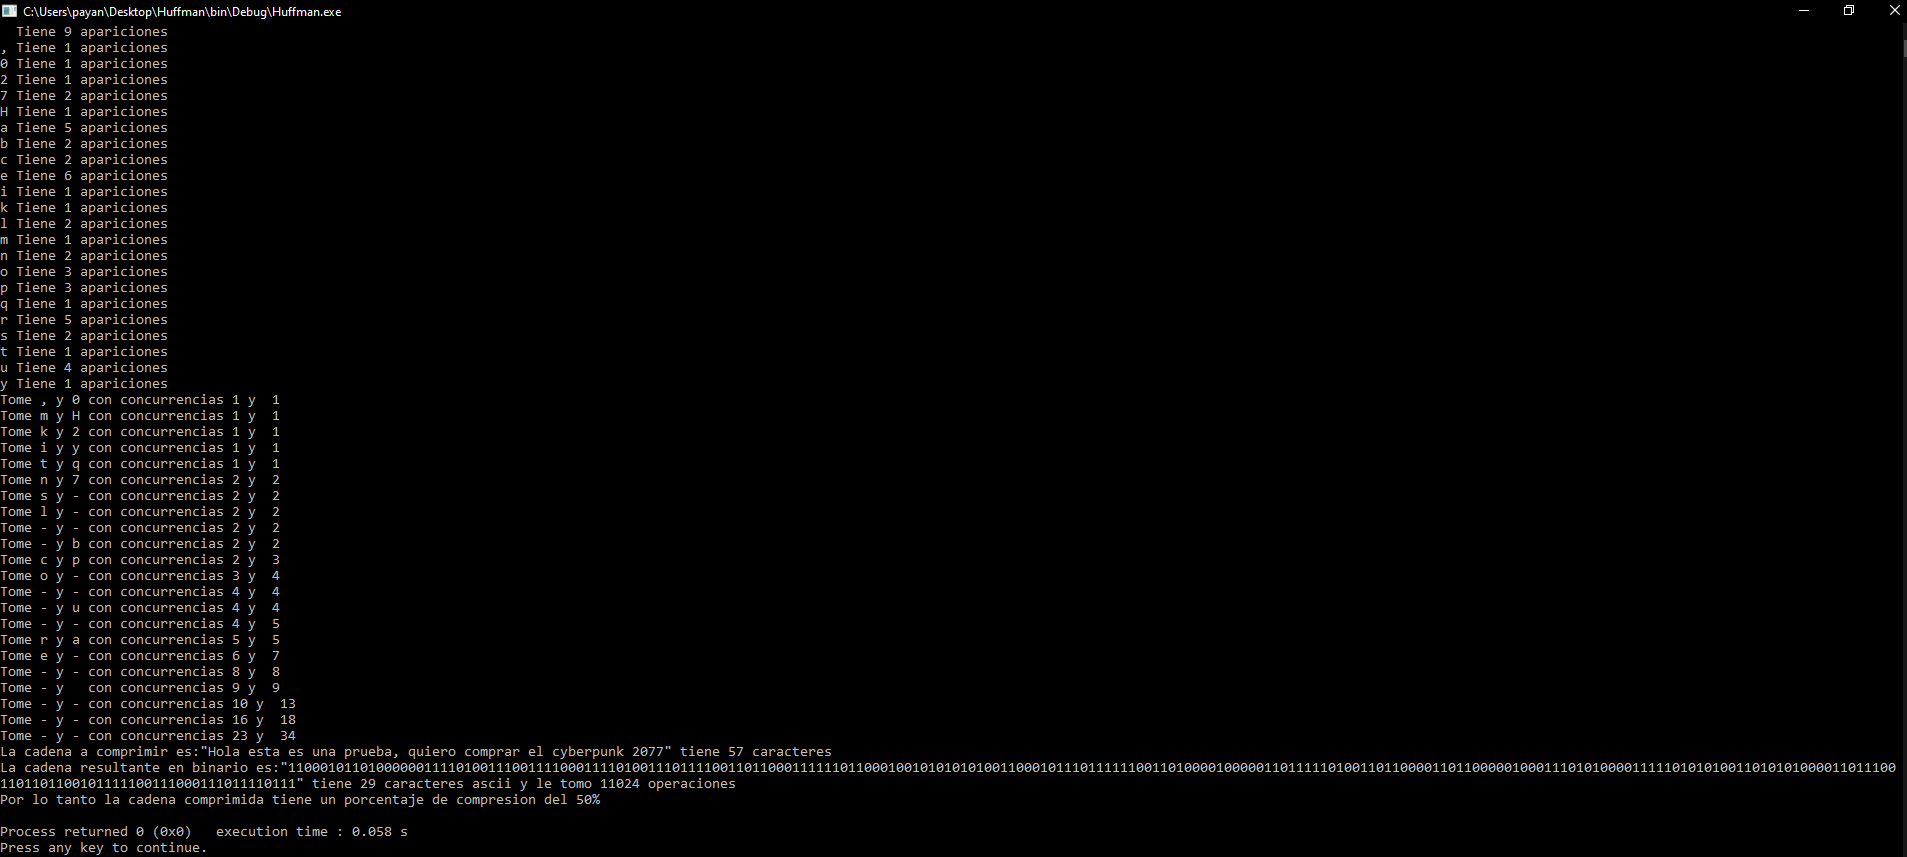
\includegraphics[width=400px,height=300px]{captura1}
		\caption{Compresión de la cadena "Hola esta es una prueba, quiero comprar el cyberpunk 2077"}
	\end{figure}
	
	\begin{figure}[H]
		\centering
		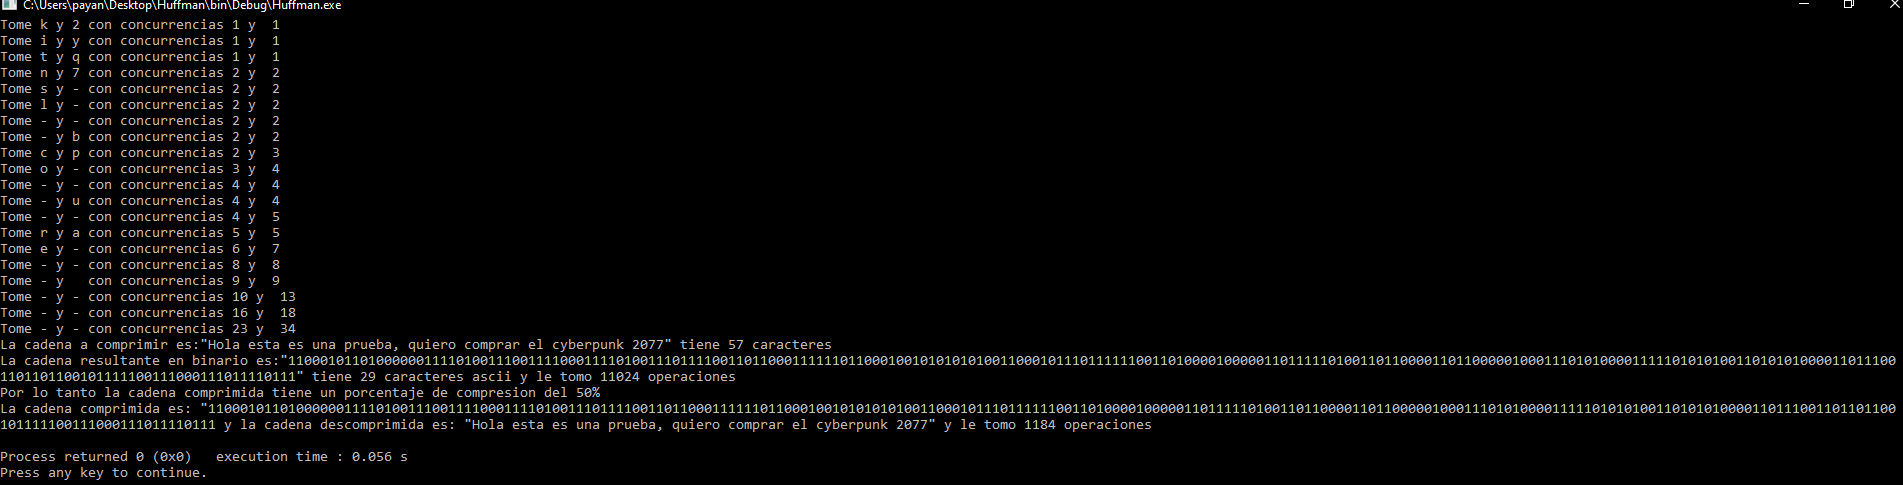
\includegraphics[width=400px,height=300px]{captura2}
		\caption{Descompresión  de la cadena "Hola esta es una prueba, quiero comprar el cyberpunk 2077"}
	\end{figure}
	Como se pudo apreciar en las capturas, la capturas, el programa tomo la entrada "Hola esta es una prueba, quiero comprar el cyberpunk 2077" y retorno la siguiente salida como respuesta: "", posteriormente al introducir la salida de la compresion en la seccion de descompresion, el programa arrojo la cadena original.
	Podemos decir que el algoritmo es eficiente, porque esta es la cantidad de caracteres de la cadena original:
	\begin{figure}[H]
		\centering
		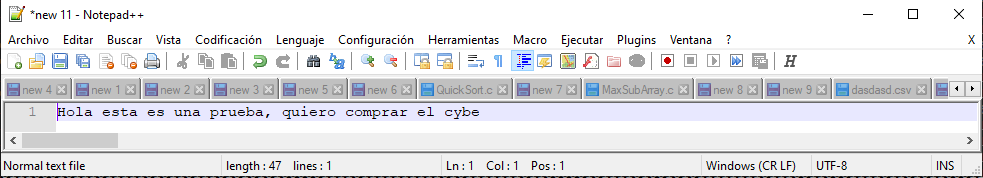
\includegraphics[width=400px,height=300px]{captura3}
		\caption{Conteo de caracteres de la entrada}
	\end{figure}
	y esta es la cantidad de caracteres de la salida:
	\begin{figure}[H]
		\centering
		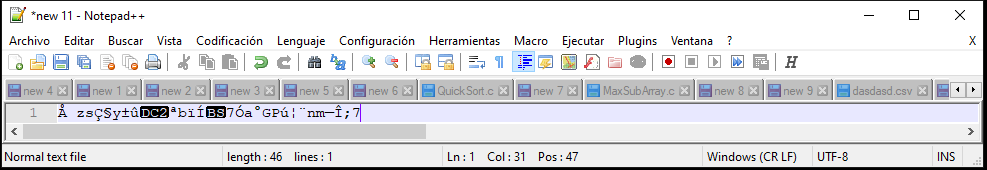
\includegraphics[width=400px,height=300px]{captura4}
		\caption{Conteo de caracteres de la salida}
	\end{figure}
	A continuacion se probo con una cadena mas larga, un "Lorem Ipsum" de 1000 bytes:
	Lorem ipsum dolor sit amet, consectetur adipiscing elit. Integer porttitor turpis eget erat auctor varius. Vestibulum maximus scelerisque dui ac vulputate. Mauris eleifend mauris vel ex sodales, ut blandit odio dictum. Ut efficitur eu lectus nec ullamcorper. Integer hendrerit justo in augue consectetur, eget porttitor quam rutrum. Cras porta justo at fermentum condimentum. Nunc lacinia convallis tortor in tempor. Donec tincidunt tempor ipsum, sit amet aliquet justo semper at. Donec nibh urna, faucibus ac mauris eu, mattis imperdiet dolor. Nam et nulla at nisi efficitur efficitur. Morbi bibendum scelerisque risus, at sollicitudin ligula rutrum et. Cras sagittis eget velit aliquam cursus.
	Nunc magna metus, ullamcorper sed ante id, tincidunt ornare libero. Proin pharetra orci felis, eget pellentesque nisi venenatis eget. Morbi tincidunt ut risus non iaculis. Proin id consectetur metus, sed placerat eros. Aenean cursus augue a ipsum tempor interdum. Vivamus viverra efficitur felis a aenean. 
	\begin{figure}[H]
		\centering
		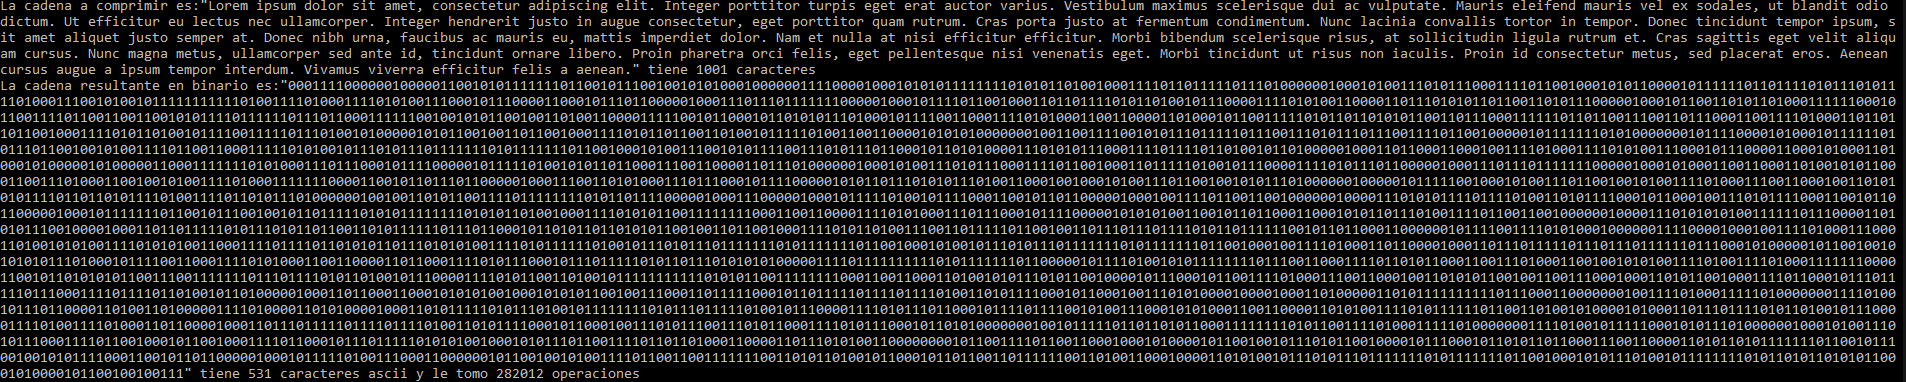
\includegraphics[width=400px,height=300px]{captura5}
		\caption{Compresión del lorem ipsum}
	\end{figure}
	
	\begin{figure}[H]
		\centering
		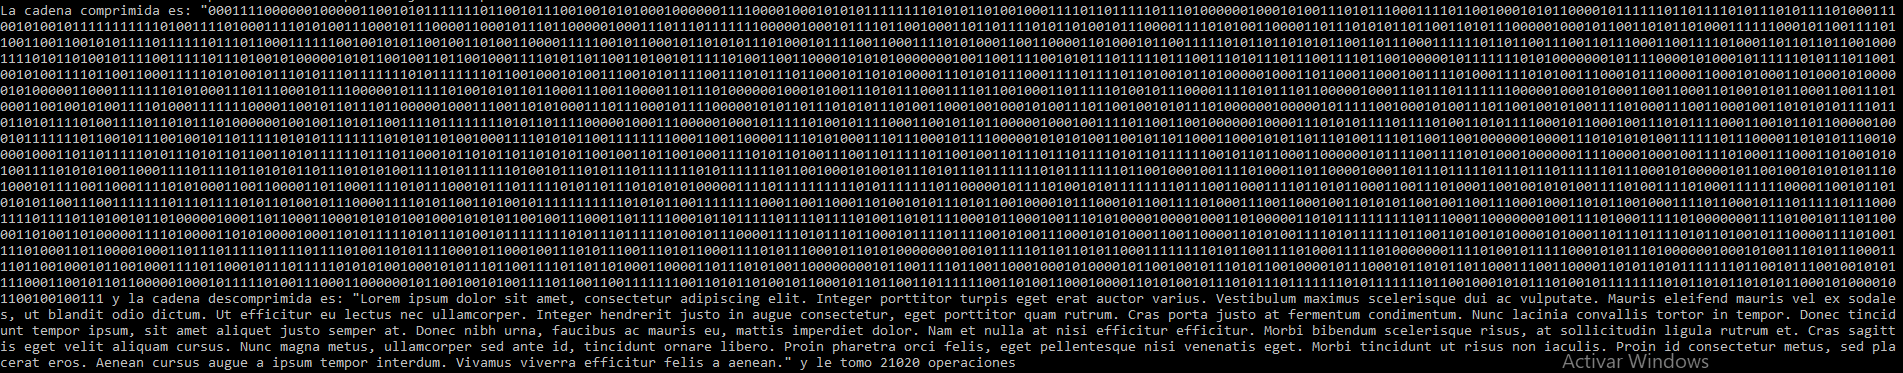
\includegraphics[width=400px,height=300px]{captura6}
		\caption{Descompresión del lorem ipsum}
	\end{figure}
	Finalmente se contaron los caractres de la entrada y de la salida:
	\begin{figure}[H]
		\centering
		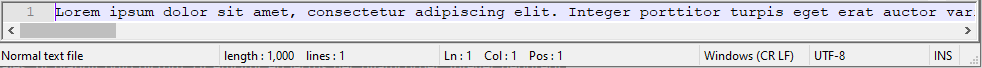
\includegraphics[width=400px,height=300px]{captura7}
		\caption{Conteo de caracteres de la entrada}
	\end{figure}
	y esta es la cantidad de caracteres de la salida:
	\begin{figure}[H]
		\centering
		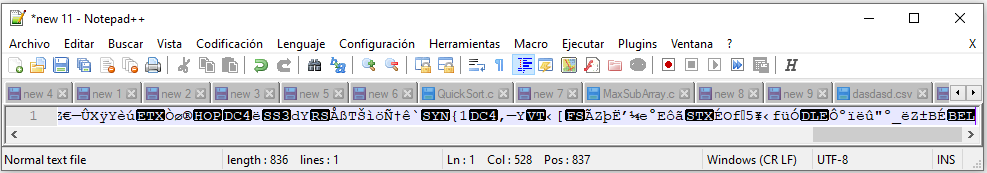
\includegraphics[width=400px,height=300px]{captura8}
		\caption{Conteo de caracteres de la salida}
	\end{figure}
	
	\begin{figure}[h!]
		\centering
		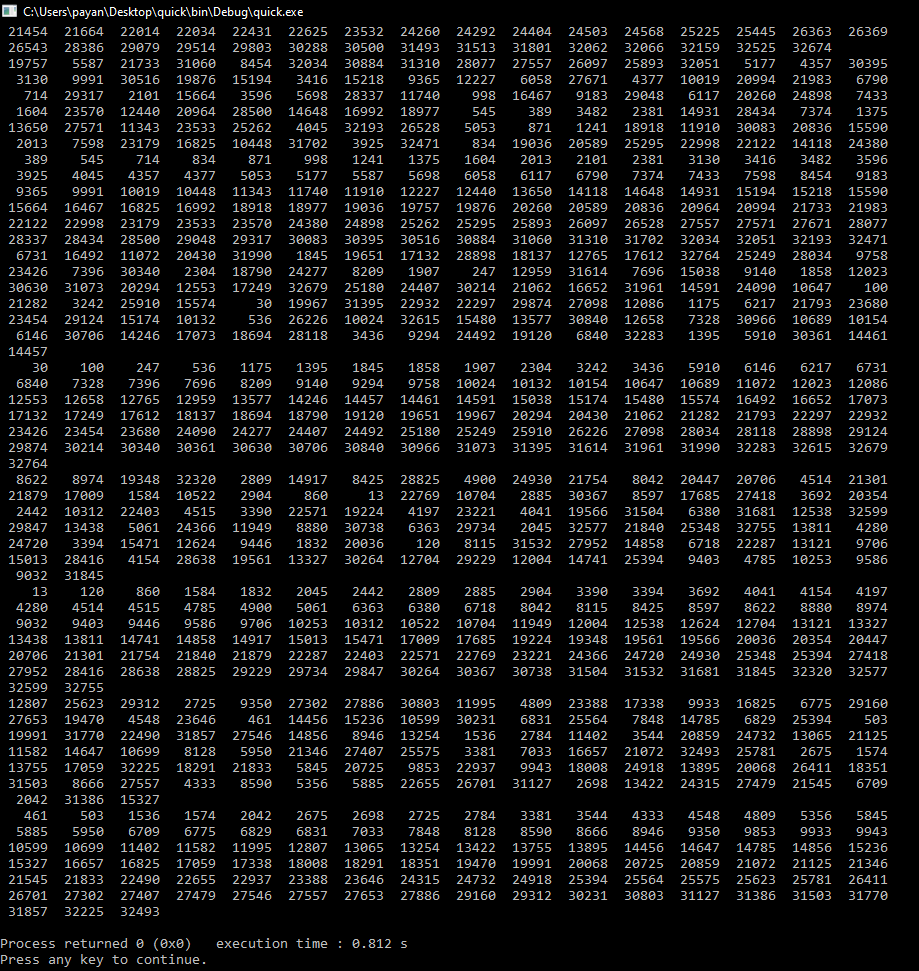
\includegraphics[width=400px,height=200px]{ejecucionPrimeraParte}
		\caption{Ejecucion del programa, Imprime el arreglo antes de ser ordenado y despues de ser ordenado, guarda en un archivo la cantidad de operaciones y el "n" para la funcion Partition (Se ejecuta en un arreglo aleatorio, aislado del ocupado por QuickSort), y los mismos datos pero para la funcion QuickSort.}
=======
	El  término  Divide  y  Vencerás  en  su  acepción  más  amplia  es  algo  más  que  una  técnica  de  diseño  de  algoritmos.  De  hecho,  suele  ser  considerada  una  filosofía  general  para  resolver  problemas  y  de  aquí  que  su  nombre  no  sólo  forme  parte  del  vocabulario informático, sino que también se utiliza en muchos otros ámbitos.      En nuestro contexto, Divide y Vencerás es una técnica de diseño de algoritmos que  consiste  en  resolver  un  problema  a  partir  de  la  solución  de  subproblemas  del  mismo tipo, pero de menor tamaño. Si los subproblemas son todavía relativamente grandes   se   aplicará   de   nuevo   esta   técnica   hasta   alcanzar   subproblemas   lo   suficientemente  pequeños  para  ser  solucionados  directamente.  Ello  naturalmente  sugiere el uso de la recursión en las implementaciones de estos algoritmos.       La  resolución  de  un  problema  mediante  esta  técnica  consta  fundamentalmente  de los siguientes pasos: 1.   En   primer   lugar   ha   de   plantearse   el   problema   de   forma   que   pueda   ser   descompuesto  en  k  subproblemas  del  mismo  tipo,  pero  de  menor  tamaño.  Es  decir, si el tamaño de la entrada es n, hemos de conseguir dividir el problema en k  subproblemas  (donde  1  ≤k≤n),  cada  uno  con  una  entrada  de  tamaño  nk  y  donde 0 ≤nk < n. A esta tarea se le conoce como división. 2.    En    segundo    lugar    han    de    resolverse    independientemente    todos    los    subproblemas,  bien  directamente  si  son  elementales  o  bien  de  forma  recursiva.  El hecho de que el tamaño de los subproblemas sea estrictamente menor que el tamaño  original  del  problema  nos  garantiza  la  convergencia  hacia  los  casos  elementales, también denominados casos base. 3.  Por  último,  combinar las soluciones obtenidas en el paso anterior para construir la solución del problema original.[1]	
	\subsection*{QuickSort}	
	\begin{algorithm}[H]
		\KwData{Entrada: N}
		\KwResult{Retorna el N-esimo termino de la serie de fibonacci}
		a=0\;
		b=0\;
		c=0\;
		\For{$i\gets1$ \KwTo $N$}{
			c = a\;
			a = b\;
			b += c\;
		}
		return a\;
		\caption{Solucion iterativa}
	\end{algorithm}
	\subsection*{Problema del maximo subarreglo}
	\begin{algorithm}[H]
		\KwData{Entrada: N}
		\KwResult{Retorna el N-esimo termino de la serie de fibonacci}
		\If{$N$ = 0}{
			return 0\;		
		}
		\ElseIf{$N$ = 1}{
			return 1\;
		}
		\Else{
			return 	solucionRecursiva($N$-1)+solucionRecursiva($N$-2);
		}
		\caption{Solucion recursiva}
	\end{algorithm}	
	\subsection*{Algoritmo de Karatsuba}	
	\section{Experimentacion y Resultados}
	\subsection{Implementar la sucecion de Fibonacci mediante un algoritmo recursivo y mediante unalgoritmo iterativo.}
	Se ejecuto el programa para encontrar los primeros 40 terminos de la sucesion de fibonacci con ambos algoritmos.			
	\begin{figure}[h!]
		\centering
		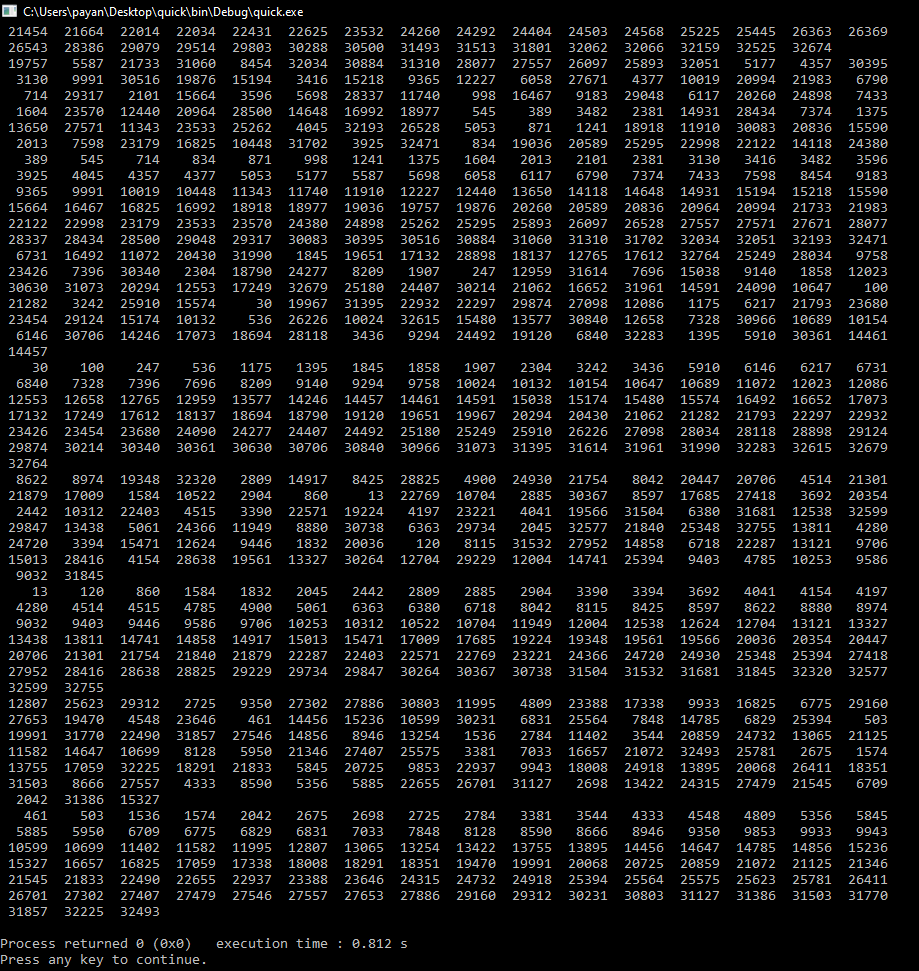
\includegraphics[width=400px,height=200px]{ejecucionPrimeraParte}
		\caption{Ejecucion del programa con ambos algoritmos, imprime $N$ y el resultado de ambas implementaciones}
	\end{figure}
	\begin{figure}[H]
		\centering
		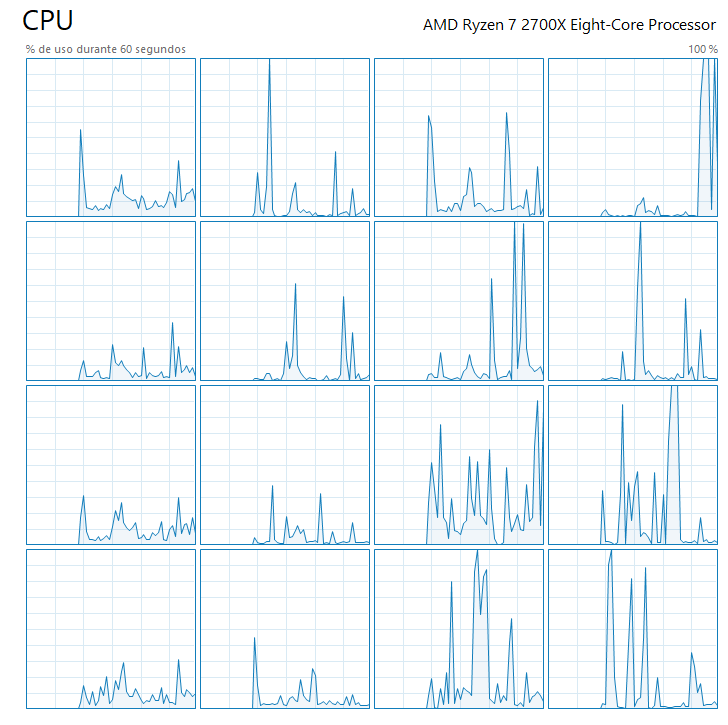
\includegraphics[width=400px,height=200px]{cpu}
		\caption{Como adicional, conforme aumentaba el valor del "limite", se incrementaba el tiempo que tardaba en terminar y el uso de CPU}
>>>>>>> 9a79e241ede170bc49baebe59f736f05ad765707
	\end{figure}
	\begin{figure}[H]
		\centering
		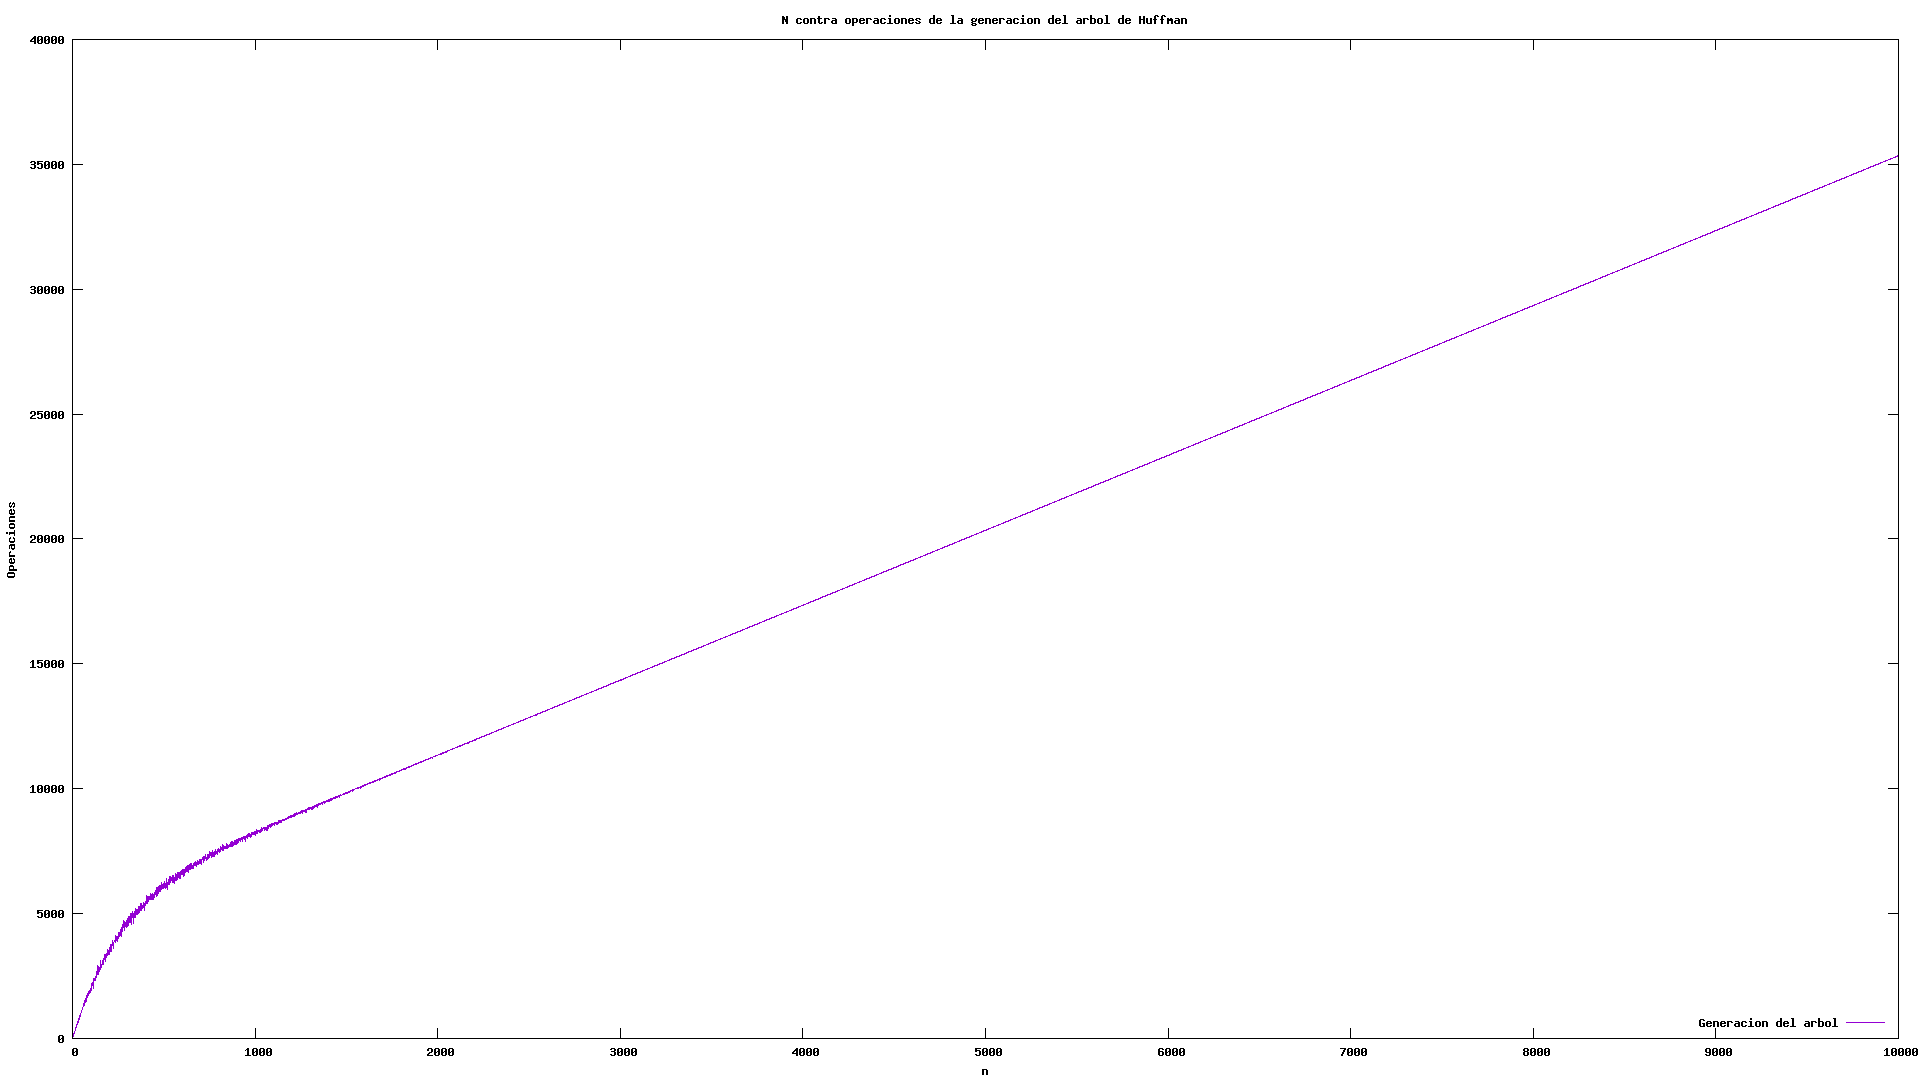
\includegraphics[width=400px,height=300px]{grafica1}
<<<<<<< HEAD
		\caption{N contra Operaciones de la funcion QuickSort en arreglos generados de forma aleatoria}
=======
		\caption{N contra Operaciones de la solucion iterativa}
>>>>>>> 9a79e241ede170bc49baebe59f736f05ad765707
	\end{figure}
	\begin{figure}[H]
		\centering
		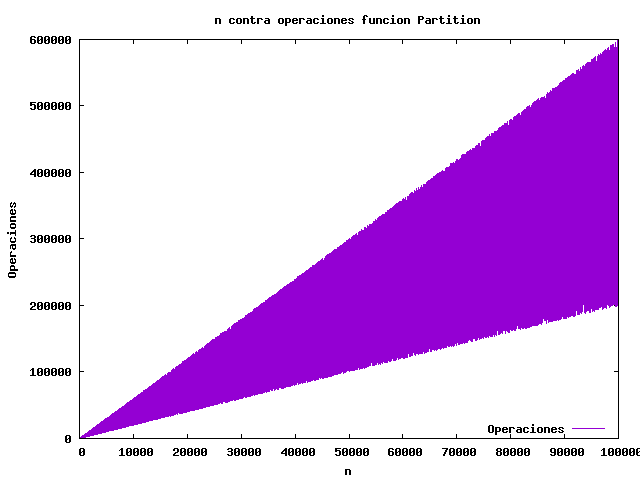
\includegraphics[width=400px,height=300px]{grafica2}
<<<<<<< HEAD
		\caption{N contra Operaciones de la funcion Partition en arreglos generados de forma aleatoria (No es el mismo arreglo que QuickSort)}
	\end{figure}	
	Ahora se procede a ejecutar la funcion QuickSort en un arreglo que contiene los numeros entre el 1 y n, donde n va desde 2 hasta 10000 ordenados de 4 formas distintas. Siendo estas:\
	\begin{enumerate}
		\item Esta ordenado de forma ascendente. Ejemplo: 1,2,3,4
		\item Esta ordenado de forma descendente. Ejemplo: 4,3,2,1
		\item Esta ordenado de forma aleatoria. Ejemplo: 2,4,1,3
		\item Esta ordenado de forma que el pivote corte el arreglo a la mitad, es decir la primera mitad del arreglo de forma ascendente y la siguiente de forma descendente. Ejemplo: 1,2,4,3
	\end{enumerate}
	\begin{figure}[H]
		\centering
		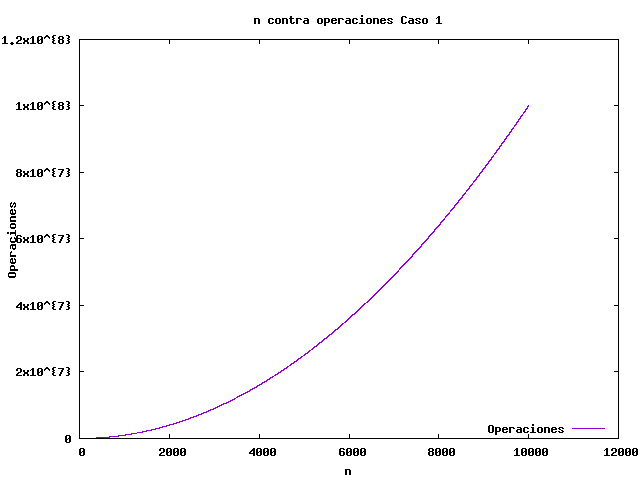
\includegraphics[width=400px,height=300px]{grafica3}
		\caption{N contra Operaciones del caso 1 de QuickSort}
	\end{figure}	
	\begin{figure}[H]
		\centering
		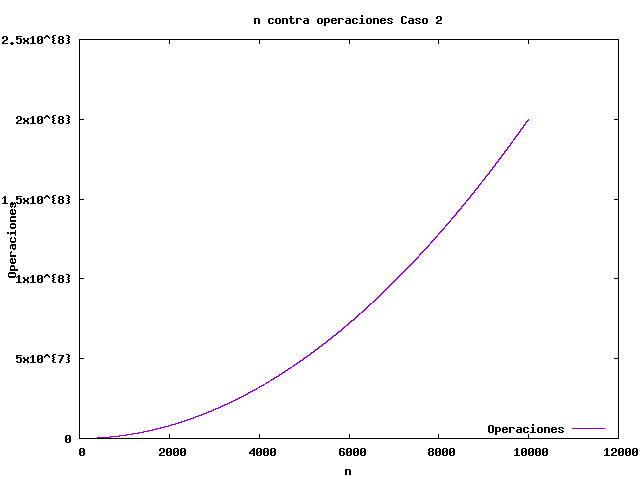
\includegraphics[width=400px,height=300px]{grafica4}
		\caption{N contra Operaciones del caso 2 de QuickSort}
	\end{figure}	
	\begin{figure}[H]
		\centering
		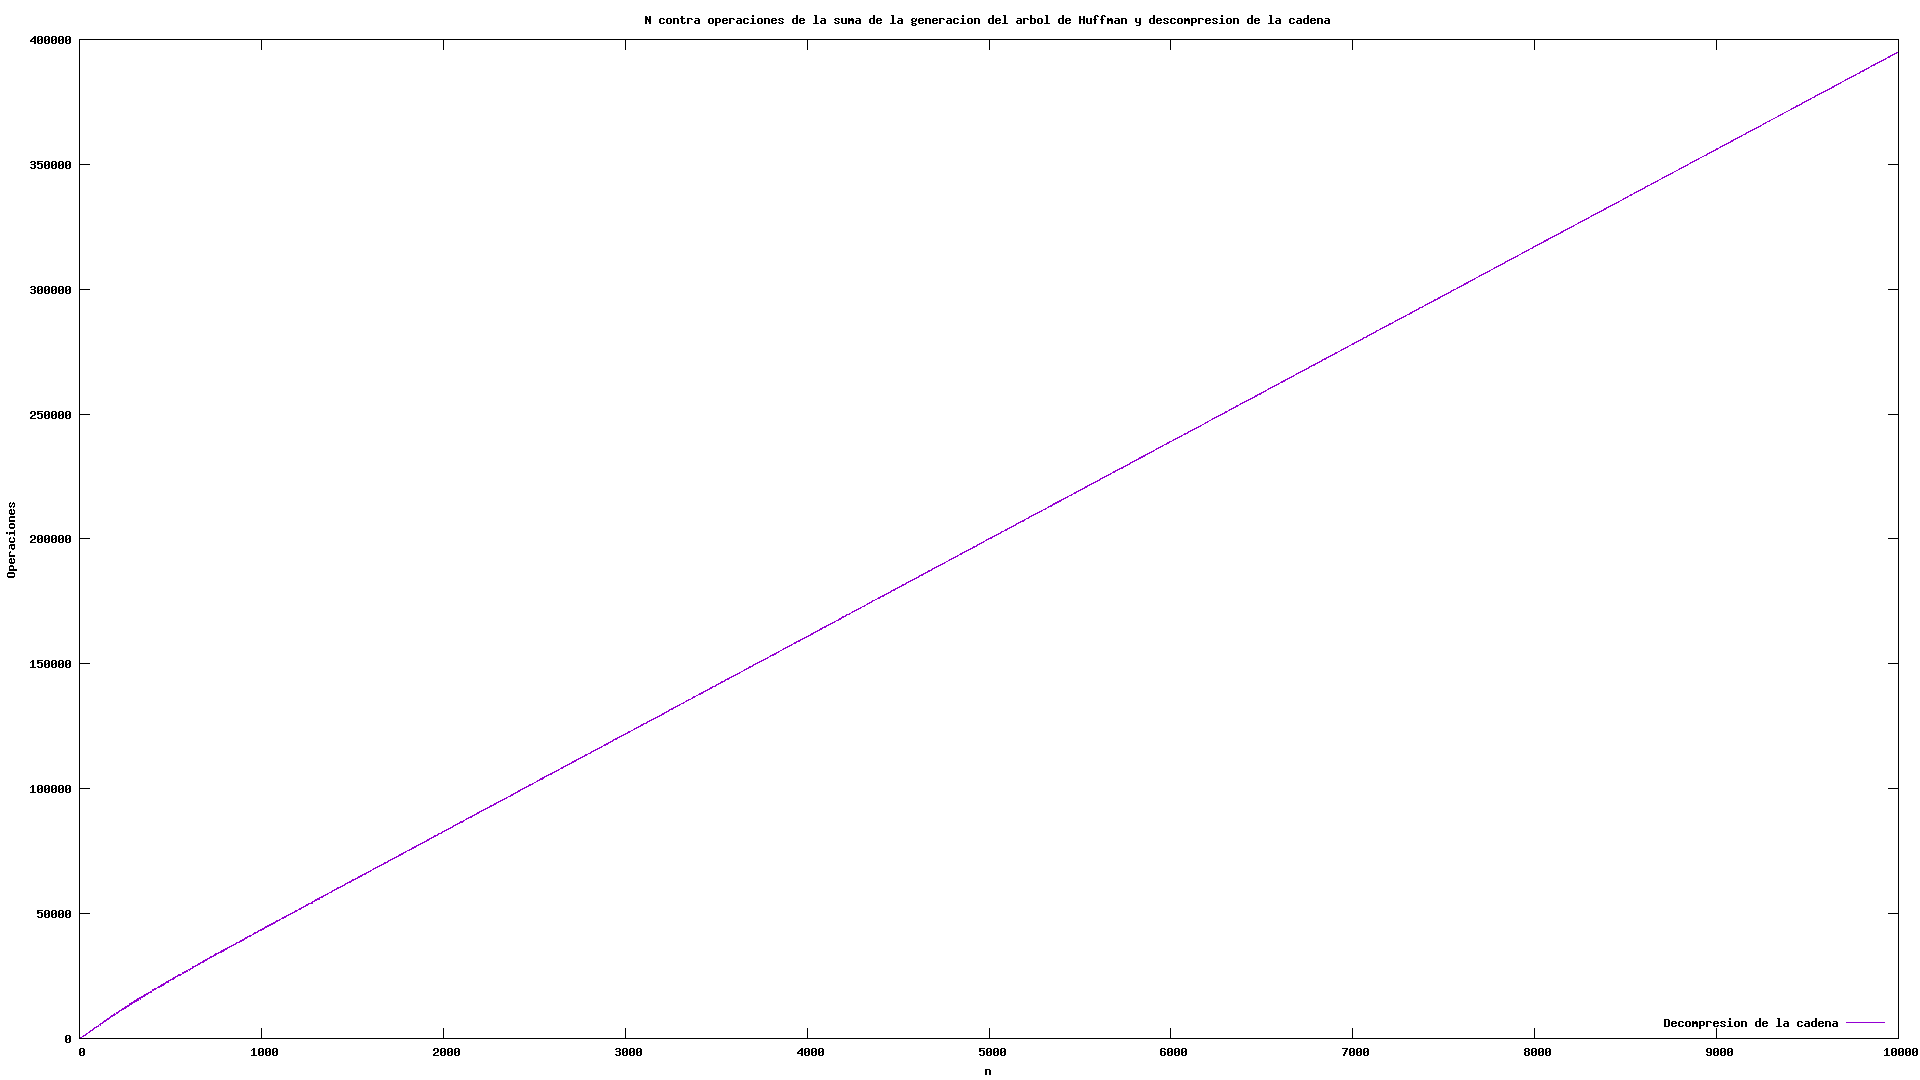
\includegraphics[width=400px,height=300px]{grafica5}
		\caption{N contra Operaciones del caso 3 de QuickSort}
	\end{figure}	
	\begin{figure}[H]
		\centering
		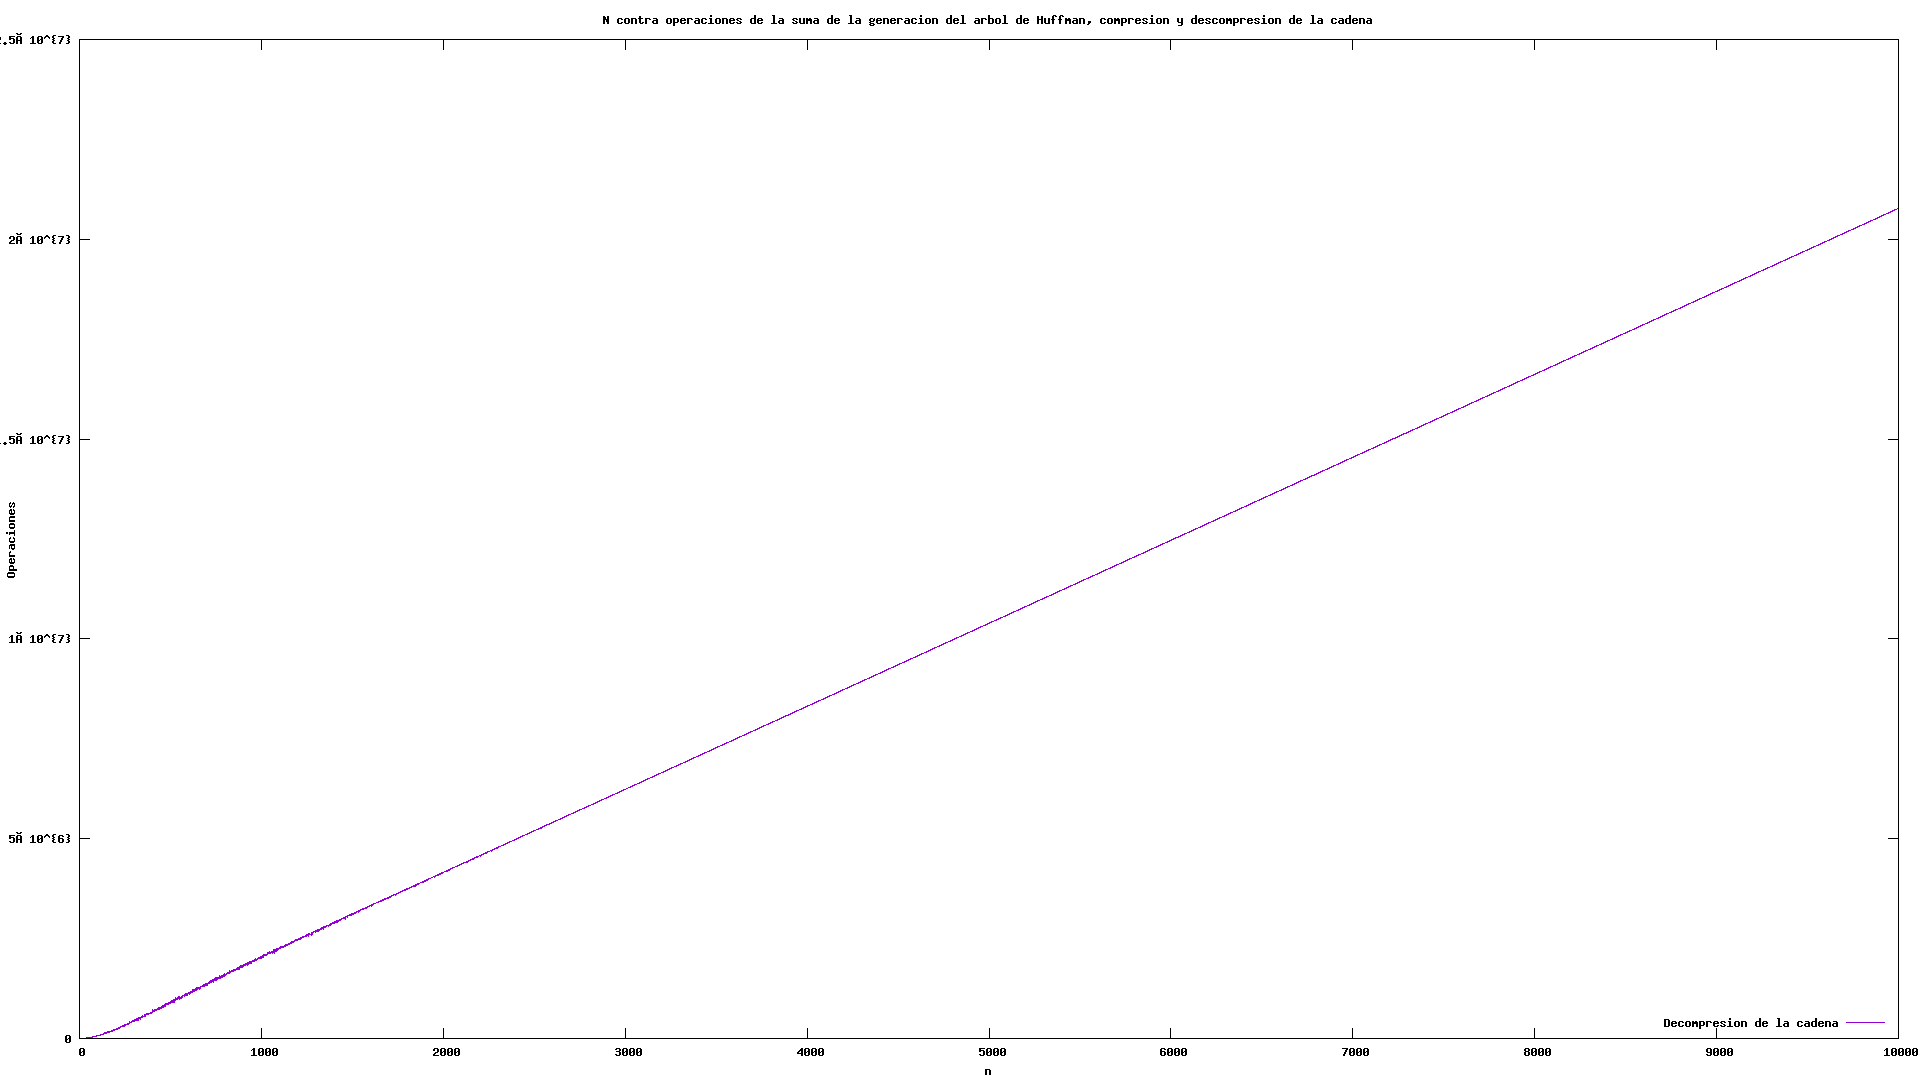
\includegraphics[width=400px,height=300px]{grafica6}
		\caption{N contra Operaciones del caso 4 de QuickSort}
	\end{figure}	
	\begin{figure}[H]
		\centering
		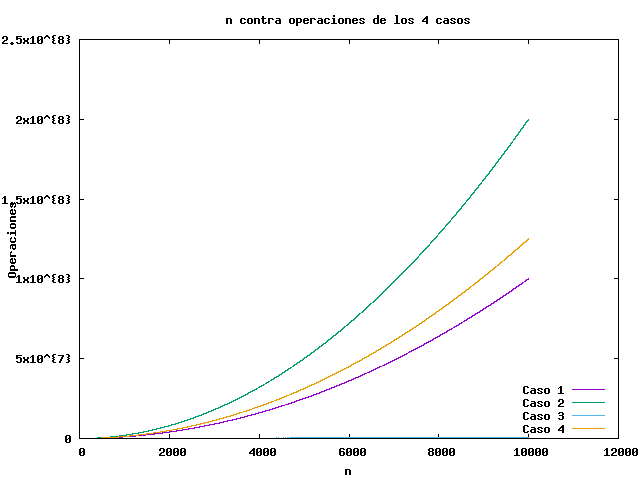
\includegraphics[width=400px,height=300px]{grafica7}
		\caption{N contra Operaciones de todos los casos combinados de QuickSort}
	\end{figure}	
	Ahora procedemos a calcular formalmente la complejidad de la funcion Partition
	Empezamos calculando la complejidad temporal de cada linea:
	\begin{center}
		\begin{table}[H]
			\begin{tabular}{|l|l|l|}
				\hline
				\rowcolor[HTML]{FFCC67} 
				Codigo                           & Costo & Veces ejecutado \\ \hline
				\textit{x = A[hasta]}                    & $\O(1)$    & 1               \\ \hline
				\textit{i = desde-1}                    & $\O(1)$    & 1               \\ \hline
				\textit{for(j=desde;j$<$hasta;j++)} & $\O(n)$    & n+1             \\ \hline
				\textit{\  \  if(A[j]<i)}                 & $\O(1)$    & n               \\ \hline
				\textit{\  \  \  \  i++}                     & $\O(1)$    & desconocido               \\ \hline
				\textit{\  \  \  \  intercambiar(A[i],A[j])}                     & $\O(3)$    & desconocido               \\ \hline
				\textit{intercambiar(A[i+1],A[hasta])}                     & $\O(3)$    & 1               \\ \hline
				\textit{return i+1}                & $\O(1)$    & 1               \\ \hline
			\end{tabular}
		\end{table}										
	\end{center}
	Esto nos indica que la complejidad de la funcion partition se ve determinada por el for que recorre desde 0 hasta n y como no es posible calcular la cantidad de veces que entrara dentro del if (ya que esto dependera del pivote), y apoyandonos por la Figure 3, podemos concluir que la funcion partition tiene complejidad $\O(n)$.\\			
	Ahora procedemos a calcular formalmente la complejidad de la funcion QuickSort (suponiendo que el pivote corta en medio del arreglo)
=======
		\caption{N contra Operaciones de la solucion recursiva}
	\end{figure}
	\begin{figure}[H]
		\centering
		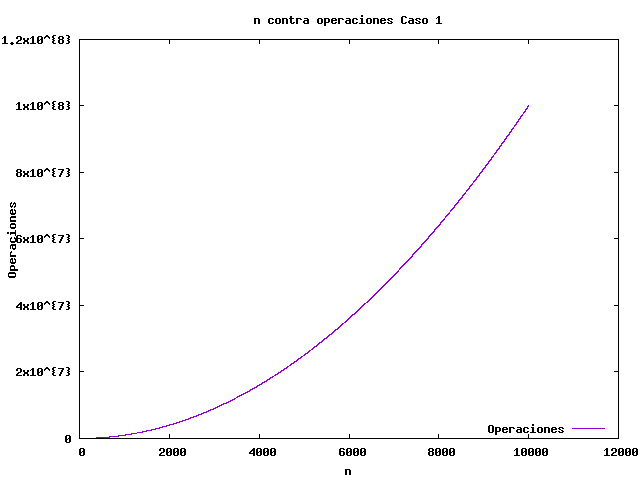
\includegraphics[width=400px,height=300px]{grafica3}
		\caption{N contra Operaciones de las dos implementaciones}
	\end{figure}
	Ahora procedemos a calcular formalmente la complejidad de la implementacion iterativa
>>>>>>> 9a79e241ede170bc49baebe59f736f05ad765707
	Empezamos calculando la complejidad temporal de cada linea:
	\begin{center}
		\begin{table}[H]
			\begin{tabular}{|l|l|l|}
				\hline
				\rowcolor[HTML]{FFCC67} 
				Codigo                           & Costo & Veces ejecutado \\ \hline
<<<<<<< HEAD
				\textit{if(desde < hasta)}                    & $\O(1)$    & 1               \\ \hline
				\textit{\  \  q = Partition(A,desde,hasta)}                    & $\O(n)$    & 1               \\ \hline
				\textit{\  \  QuickSort(A,desde,q-1)}                    & $T(\frac{n}{2})$    & 1               \\ \hline						
				\textit{\  \  QuickSort(A,q+1,hasta)}                    & $T(\frac{n}{2})$    & 1               \\ \hline						
			\end{tabular}
		\end{table}										
	\end{center}
	Bajo este escenario que coincide con el caso 4 de los analisis respecto a QuickSort (Figure 7) obtenemos la siguiente ecuacion de recurrencia:\\
	$T(n) = 2T(\frac{n}{2})+\O(n)$\\
	Que al ser desarrollada llegaremos a la conclusion de que: $T(n)$ tiene complejidad $\Theta(nlog_2(n))$.\\
	Ahora bien, para los otros 3 escenarios la cosa cambia bastante, si miramos la figure 4 podemos ver que el comportamiento de la funcion se torna cuadratico, muy similar al escenario 2 (Figure 5), ya que generamos casos donde el arreglo es dividido en 0 y n elementos, lo cual vuelve la complejidad del ordenamiento cuadratica.\\
	Pero tomando el caso de números aleatorios (Figure 6 y Figure 2) podemos ver que en la mayoria de los casos, el algoritmo tendra complejidad $\O(nlog_2(n))$, aunque dependera de la implementación, en este caso se tomo el pivote como el ultimo valor del arreglo, lo cual es puede ser poco eficiente, por ello se recomienda tomar valores como la media o mediana.\\
	\subsection{Implementar el algoritmo del Maximo SubArreglo}
	Para este algoritmo se decidio generar un arreglo aleatorio de n elementos (n va de 1 hasta 10000), y medir la complejidad del algoritmo de fuerza bruta y del algoritmo de divide y venceras.
=======
				\textit{a = 0}                    & $\O(1)$    & 1               \\ \hline
				\textit{b = 0}                    & $\O(1)$    & 1               \\ \hline
				\textit{c = 0}                    & $\O(1)$    & 1               \\ \hline						
				\textit{for(i=0;i$\leq$n;i++)} & $\O(n)$    & n+2             \\ \hline
				\textit{\  \  c = a}                 & $\O(1)$    & n               \\ \hline
				\textit{\  \  a = b}                     & $\O(1)$    & n+1               \\ \hline
				\textit{\  \  b += c}                     & $\O(1)$    & n+1               \\ \hline
				\textit{return a}                & $\O(1)$    & 1               \\ \hline
			\end{tabular}
		\end{table}										
	\end{center}			
	Lo cual nos indica que la complejidad de la solucion iterativa es lineal, es decir $T(n)\in\O(n)$. Esto lo podemos corroborar en la Figure 3 donde se puede apreciar que el numero de operaciones de la implementacion contra N crece de forma lineal.\\			
	Por otro lado, de forma experimental podemos proponer que la complejidad de la solución recursiva es: $2^N$			
	\subsection{Implementar las funciones Perfecto(N) y MostrarPerfectos(N)}
	Para el segundo conjunto de funciones, se decidio buscar los primeros 4 números perfectos, y probar todos los números hasta 10 000.
>>>>>>> 9a79e241ede170bc49baebe59f736f05ad765707
	\begin{figure}[H]
		\centering
		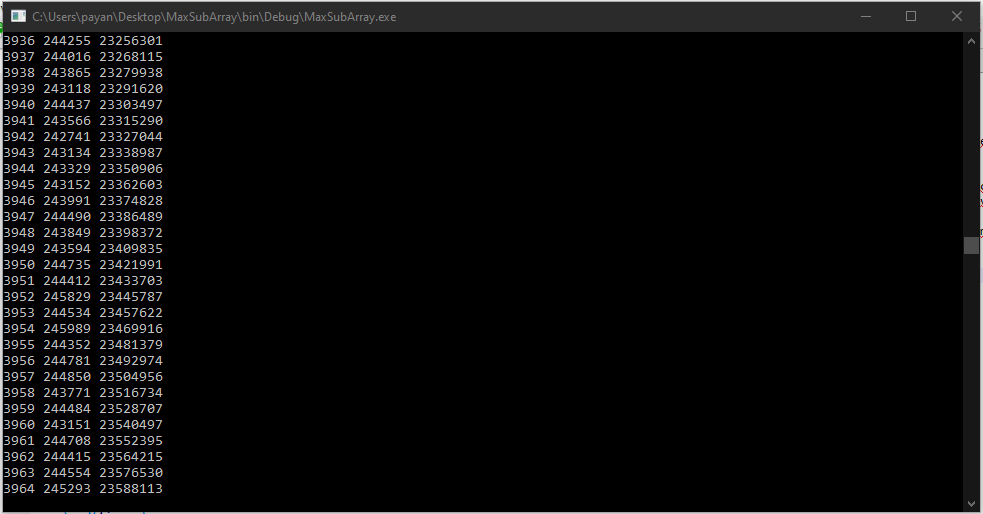
\includegraphics[width=400px,height=200px]{ejecucionSegundaParte}
		\caption{Ejecucion del programa en la seccion de prueba de números}
	\end{figure}
	\begin{figure}[H]
		\centering
<<<<<<< HEAD
		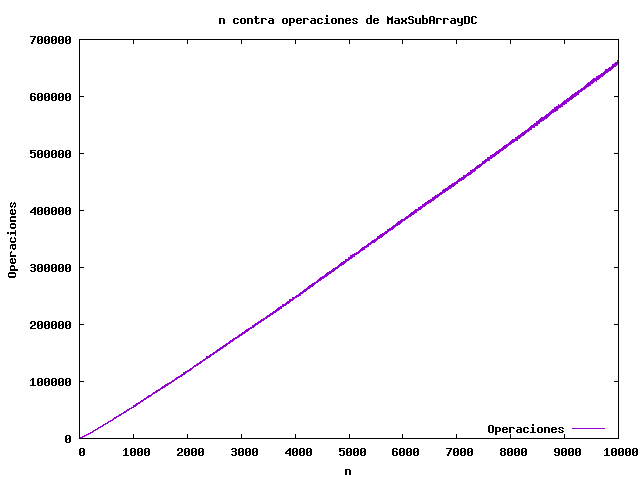
\includegraphics[width=400px,height=300px]{grafica8}
		\caption{N contra Operaciones de MaxSubArrayDC en arreglos aleatorios de tamaño n}
	\end{figure}
	\begin{figure}[H]
		\centering
		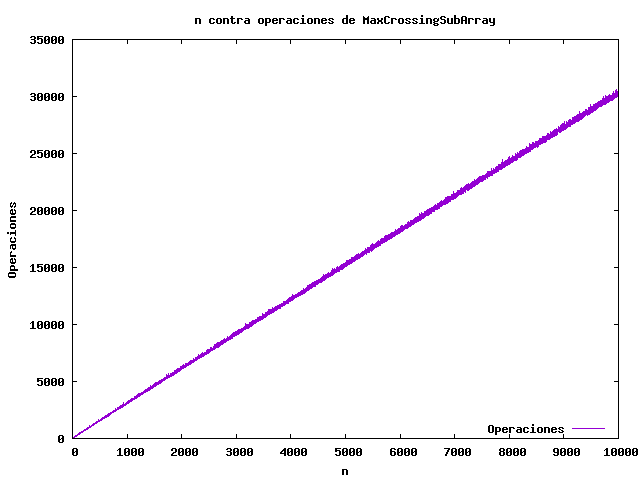
\includegraphics[width=400px,height=300px]{grafica9}
		\caption{N contra Operaciones de MaxCrossingSubArray en arreglos aleatorios de tamaño n}
	\end{figure}
	\begin{figure}[H]
		\centering
		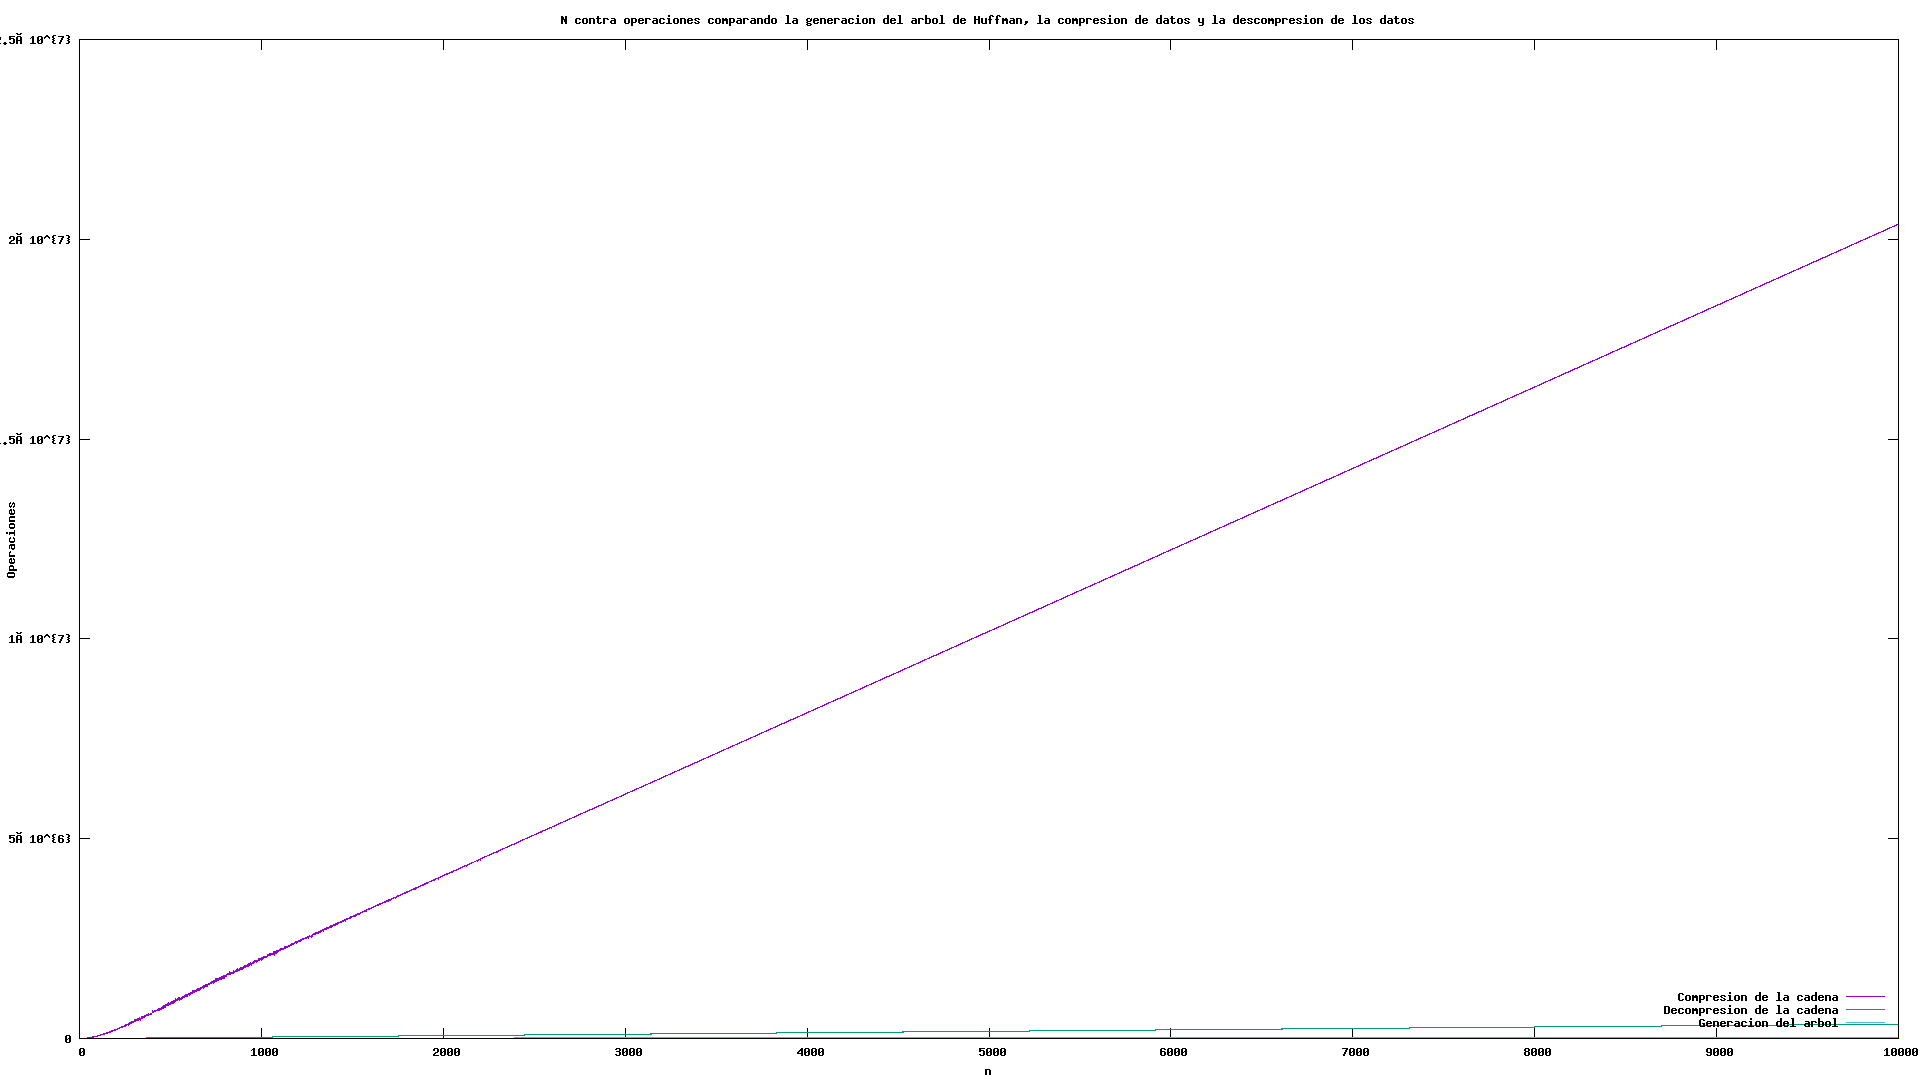
\includegraphics[width=400px,height=300px]{grafica10}
		\caption{N contra Operaciones de FuerzaBruta en arreglos aleatorios de tamaño n}
	\end{figure}
	\begin{figure}[H]
		\centering
		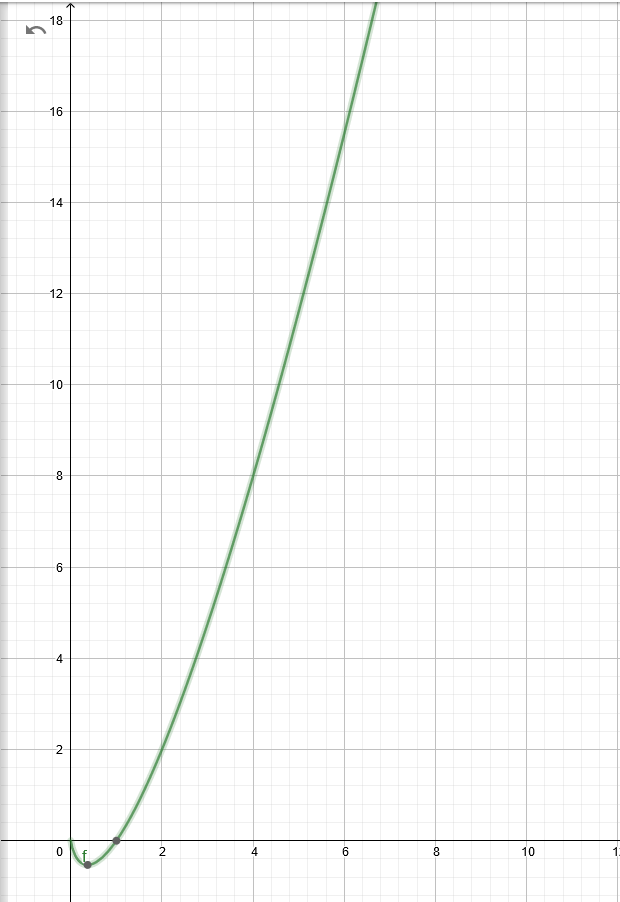
\includegraphics[width=400px,height=300px]{grafica11}
		\caption{N contra Operaciones de MaxSubArrayDC y FuerzaBruta combinados en arreglos aleatorios de tamaño n}
	\end{figure}
	Ahora procederemos a calcular formalmente la complejidad de la funcion MaxCrossingSubArray:
=======
		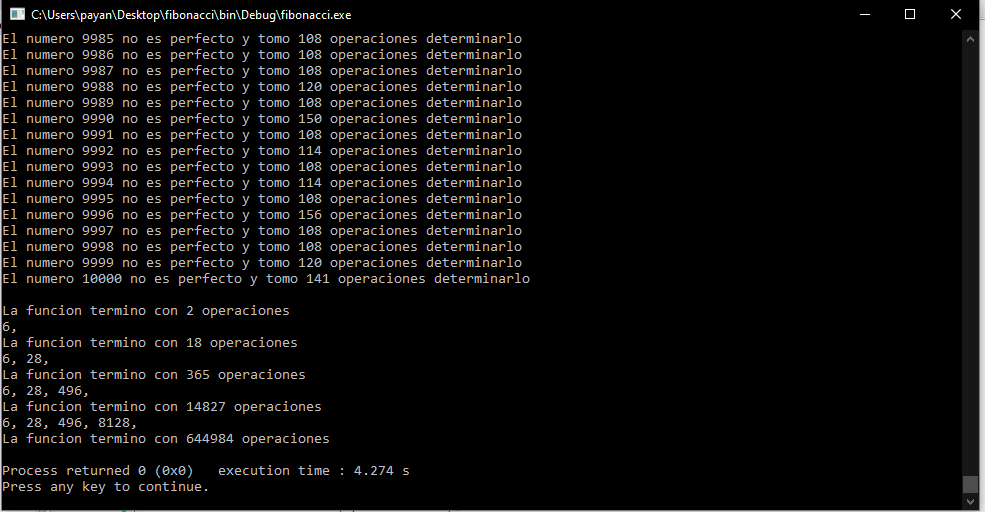
\includegraphics[width=400px,height=200px]{ejecucionTerceraParte}
		\caption{Ejecucion del programa en la seccion de obtener N perfectos}
	\end{figure}
	\begin{figure}[h!]
		\centering
		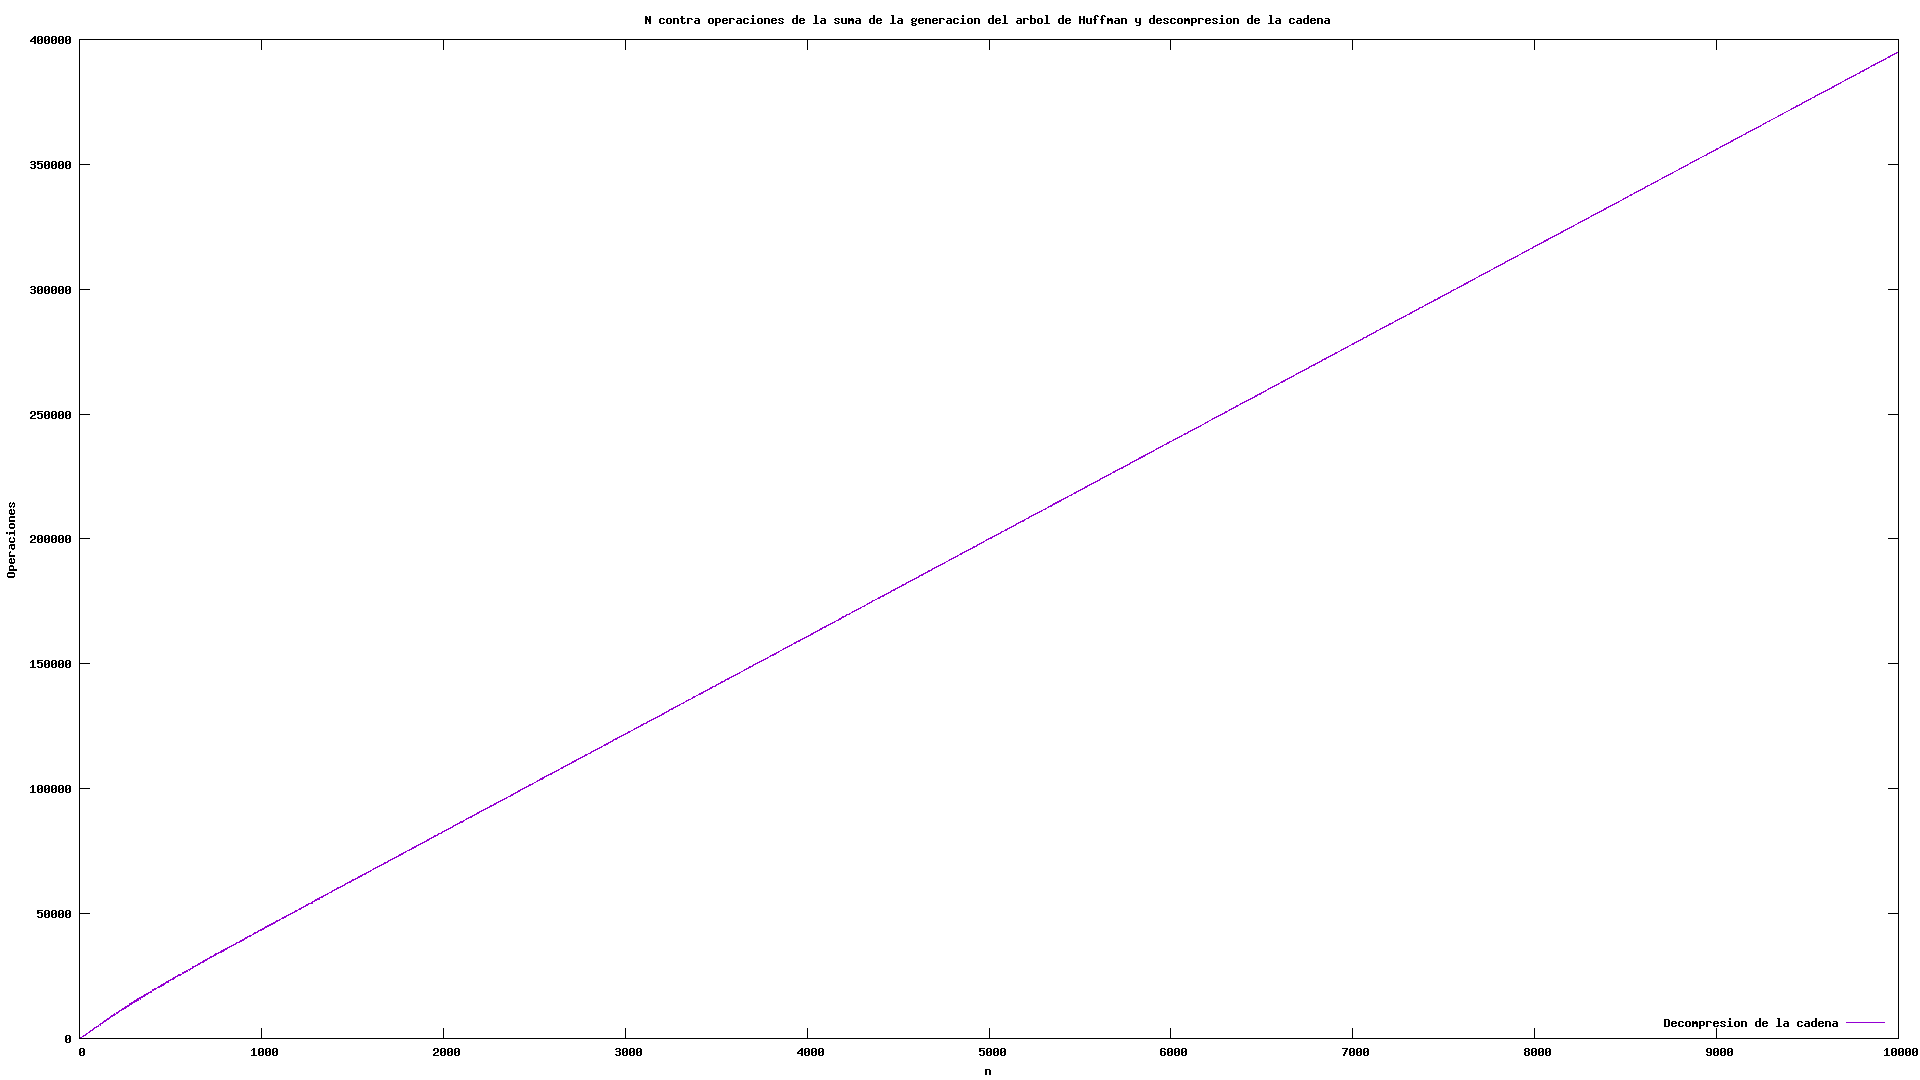
\includegraphics[width=400px,height=300px]{grafica5}
		\caption{N contra Operaciones de Perfecto(N)}
	\end{figure}
	\begin{figure}[H]
		\centering
		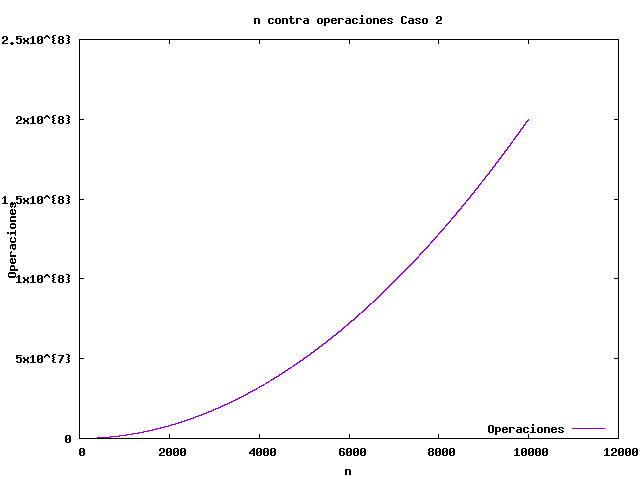
\includegraphics[width=400px,height=300px]{grafica4}
		\caption{N contra Operaciones de MostrarPerfectos(N)}
	\end{figure}
	Ahora procedemos a calcular formalmente la complejidad de la funcion Perfecto(N)
	Empezamos calculando la complejidad temporal de cada linea:
>>>>>>> 9a79e241ede170bc49baebe59f736f05ad765707
	\begin{center}
		\begin{table}[H]
			\begin{tabular}{|l|l|l|}
				\hline
				\rowcolor[HTML]{FFCC67} 
				Codigo                           & Costo & Veces ejecutado \\ \hline
<<<<<<< HEAD
				\textit{suma, suma$\_$izq, suma$\_$der}                    & $\O(1)$    & 1               \\ \hline
				\textit{max$\_$izq = max$\_$der = INT$\_$MIN;}                    & $\O(1)$    & 1               \\ \hline								
				\textit{for(i=mitad;i$\geq$bajo;i--)} & $\O(1)$    & $\frac{n}{2}+1$             \\ \hline
				\textit{\  \  suma+=arreglo[i]}                 & $\O(1)$    & $\frac{n}{2}$               \\ \hline
				\textit{\  \  if(suma$>$suma$\_$izq)}                 & $\O(1)$    & $\frac{n}{2}$               \\ \hline
				\textit{\  \  \  \  max$\_$izq=i}                     & $\O(1)$    & indefinido              \\ \hline
				\textit{\  \  \  \  suma$\_$izq=suma}                     & $\O(1)$    & indefinido              \\ \hline				
				\textit{for(i=mitad+1;i$<$alto;i++)} & $\O(1)$    & $\frac{n}{2}$+1             \\ \hline
				\textit{\  \  suma+=arreglo[i]}                 & $\O(1)$    & $\frac{n}{2}$               \\ \hline
				\textit{\  \  if(suma$>$suma$\_$der)}                 & $\O(1)$    & $\frac{n}{2}$               \\ \hline
				\textit{\  \  \  \  max$\_$der=i}                     & $\O(1)$    & indefinido              \\ \hline
				\textit{\  \  \  \  suma$\_$der=suma}                     & $\O(1)$    & indefinido              \\ \hline			
				\textit{return(suma$\_$izq+suma$\_$der,max$\_$izq,max$\_$der)}                     & $\O(1)$    & 1              \\ \hline			
			\end{tabular}
		\end{table}										
	\end{center}			
	Al analizar la complejidad linea a linea y apoyado por la grafica "Figure 11" , podemos decir que la complejidad de la funcion es $O(n)$.
	Una vez que tenemos este dato, procedemos a analizar la complejidad de la funcion MaxSubArrayDC:
	\begin{center}
		\begin{table}[H]
			\begin{tabular}{|l|l|l|}
				\hline
				\rowcolor[HTML]{FFCC67} 
				Codigo                           & Costo & Veces ejecutado \\ \hline
				\textit{suma, suma$\_$izq, suma$\_$der}                    & $\O(1)$    & 1               \\ \hline
				\textit{max$\_$izq = max$\_$der = INT$\_$MIN;}                    & $\O(1)$    & 1               \\ \hline								
				\textit{for(i=mitad;i$\geq$bajo;i--)} & $\O(1)$    & $\frac{n}{2}+1$             \\ \hline
				\textit{\  \  suma+=arreglo[i]}                 & $\O(1)$    & $\frac{n}{2}$               \\ \hline
				\textit{\  \  if(suma$>$suma$\_$izq)}                 & $\O(1)$    & $\frac{n}{2}$               \\ \hline
				\textit{\  \  \  \  max$\_$izq=i}                     & $\O(1)$    & indefinido              \\ \hline
				\textit{\  \  \  \  suma$\_$izq=suma}                     & $\O(1)$    & indefinido              \\ \hline				
				\textit{for(i=mitad+1;i$<$alto;i++)} & $\O(1)$    & $\frac{n}{2}$+1             \\ \hline
				\textit{\  \  suma+=arreglo[i]}                 & $\O(1)$    & $\frac{n}{2}$               \\ \hline
				\textit{\  \  if(suma$>$suma$\_$der)}                 & $\O(1)$    & $\frac{n}{2}$               \\ \hline
				\textit{\  \  \  \  max$\_$der=i}                     & $\O(1)$    & indefinido              \\ \hline
				\textit{\  \  \  \  suma$\_$der=suma}                     & $\O(1)$    & indefinido              \\ \hline			
				\textit{return(suma$\_$izq+suma$\_$der,max$\_$izq,max$\_$der)}                     & $\O(1)$    & 1              \\ \hline			
			\end{tabular}
		\end{table}										
	\end{center}
	Terminado el analisis, obtendremos que la complejidad esta determinada por la siguiente ecuacion de recurrencia: $T(n) = 2T(\frac{n}{2})+\O(n)$, una vez resuelta, determinaremos que la complejidad final de la funcion MaxSubArrayDC es $\O(nlog_2(n))$ esto lo podemos respaldar con las Figure 10 y Figure 13 , en las cuales se aprecia que la complejidad de la funcion esta acotada por $\O(nlog_2(n))$.
	Finalmente como contraste se analizara la funcion FuerzaBruta:
	\begin{center}
		\begin{table}[H]
			\begin{tabular}{|l|l|l|}
				\hline
				\rowcolor[HTML]{FFCC67} 
				Codigo                           & Costo & Veces ejecutado \\ \hline
				\textit{sumaLocal, lIndex, rIndex = 0}                    & $\O(1)$    & 1               \\ \hline
				\textit{suma = INT$\_$MAX}                    & $\O(1)$    & 1               \\ \hline				

				\textit{for(i=0;i$<$n;i++)} & $\O(1)$    & $n+1$             \\ \hline
				\textit{\  \  sumaLocal=0}                 & $\O(1)$    & $n$               \\ \hline
				\textit{\  \  for(j=i;j$<$n;j++)}                 & $\O(1)$    & $n$               \\ \hline
				\textit{\  \  \  \  if(sumaLocal$>$suma)}                     & $\O(1)$    & $\frac{(n)(n-1)}{2}+1$              \\ \hline
				\textit{\  \  \  \  \  \  suma = sumaLocal}                     & $\O(1)$    & indefinido              \\ \hline				
				\textit{\  \  \  \  \  \  lIndex = i}                     & $\O(1)$    & indefinido              \\ \hline				
				\textit{\  \  \  \  \  \  rIndex = j}                     & $\O(1)$    & indefinido              \\ \hline								
				\textit{return(suma,lIndex,rIndex)}                     & $\O(1)$    & 1              \\ \hline			
			\end{tabular}
		\end{table}										
	\end{center}
	Al terminar el analisis podemos ver que la complejidad de la funcion es $\O(n^2)$ lo cual coincide bastante con lo que se aprecia en las graficas (Figure 12 y Figure 13).

	
	\section{Conclusiones}			
	\subsection{Payán Téllez René}
	Despues de analizar los algoritmos del maximo sub arreglo y del QuickSort, puedo concluir que la tecnica de divide y venceras es extremadamente potente y sirve para resolver problemas que de otra forma tomarian mucha mas complejidad computacional, por ejemplo la funcion FuerzaBruta y el BubbleSort son prueba de ello ya que estos algoritmos que implementan soluciones mas directas, tienen complejidades enormes. Por otro lado no todo es perfecto, ya que en el caso particular del QuickSort, pude apreciar que la complejidad podia crecer hasta ser extremadamente ineficiente en casos donde el arreglo este ordenado de tal forma que el pivote no corte nada del mismo, aunque analizando a profundidad estos casos pueden ser diezmados y en ciertas implementaciones que me encontre en la web, se toman varias medidas para hacerlo, como aleatorizar el arreglo o buscar un pivote mas optimo.\\
	\includegraphics[height=120px,width=120px]{Rene}
	\section{Anexo}			
	\subsection{Investigar el algoritmo de Karatsuba que permite obtener la multiplicación de enteros muy grandes}
	Resuelto, se encuentra en los conceptos basicos
	\subsection{Resolver los siguientes problemas}
	\section{Bibliografia}
		{[}1{]}\url{https://openwebinars.net/blog/que-es-un-algoritmo-informatico/}\\
		{[}2{]}\url{http://www.lcc.uma.es/~av/Libro/CAP3.pdf}\\
		{[}3{]}\url{https://es.qaz.wiki/wiki/Karatsuba_algorithm}\\
=======
				\textit{raiz = sqrt(n)}                    & $\O(1)$    & 1               \\ \hline
				\textit{suma = 1}                    & $\O(1)$    & 1               \\ \hline
				\textit{for(i=2;i$\leq$raiz;i++)} & $\O(\sqrt{n})$    & $\sqrt{n}$+2             \\ \hline
				\textit{\  \  if(n mod i == 0)}                 & $\O(1)$    & $\sqrt{n}$               \\ \hline
				\textit{\  \  \  \  if(n/i > raiz)}                     & $\O(log_2(n))$    & $log_2(n)+1$              \\ \hline
				\textit{\  \  \  \  \  \  suma += n/i}                     & $\O(1)$    & $\frac{log_2(n)}{2}$               \\ \hline
				\textit{\  \  \  \  suma+=i}                     & $\O(1)$    & $log_2(n)$               \\ \hline
				\textit{return (suma==n?1:0)}                & $\O(1)$    & 1               \\ \hline
			\end{tabular}
		\end{table}										
	\end{center}			
	Lo cual nos indica que la complejidad de la funcion Perfecto(n) es $\sqrt{n}$, es decir $T(n)\in\O(\sqrt{n})$. Esto lo podemos corroborar en la Figure 3 donde se puede apreciar que el numero de operaciones de la implementacion contra N crece acotado por abajo por $\sqrt(2)$ y acotado por arriba por $c\sqrt{n}$.\\			
	Por otro lado, de forma experimental y basado en la tabla de perfectos conocidos,podemos observar que la complejidad de la funcion MostrarPerfectos(n) crece de forma exponencial debido a que el espacio entre cada perfecto es muy grande, asimismo las formas mas optimas que ocupan el calculo de un primo p, igual tienen complejidades gigantes, debido a que es dificil hallar un primo y no todos aplican para la funcion, sin mencionar que computacionalmente cuesta muchisimo trabajo hacerlo.
	
	\section{Conclusiones}			
	\subsection{Payán Téllez René}
	Esta practica se me hizo particulamente interesante porque los algoritmos que se trataron, no fueron tan directos de implementar en un lenguaje de programación, sin mencionar que algunas graficas tuvieron muy pocos valores, debido a lo complicado que era generar mas, porque computacionalmente su complejidad es inmensa. De hecho tuve que cambiar algunas variables de int a long long int en el espacio de los contadores para que siguiera funcionando el contador sin desbordarse. Tambien vi lo interesante de un algoritmo como MostrarPerfectos que tiene una complejidad no polinomial, ya que aunque lo puedo programar tardaria horas en encontrar mas alla del perfecto 5 (de por si toma mas de 5 minutos hallar el perfecto 4) sin mencionar que le tomaria dias encontrar otros números. Tambien cuando estaba demostrando la complejidad del algoritmo recursivo de la secuencia de fibonacci, algunos nucleos del CPU de mi computadora se dispararon, lo cual fue una señal de lo complicado y tardado que se podia volver en N muy grandes.\\
	\includegraphics[height=120px,width=120px]{Rene}
	\section{Anexo}			
	\subsection{Investigar el algoritmo de Karatsuba que permite obtener la multiplicación de enteros muy grandes}
	\subsection{Resolver los siguientes problemas}
	\section{Bibliografia}
		{[}1{]}\url{http://www.lcc.uma.es/~av/Libro/CAP3.pdf}\\
		{[}2{]}\url{https://medium.com/@joseguillermo_/qu\%C3\%A9-es-la-complejidad-algor\%C3\%ADtmica-y-con-qu\%C3\%A9-se-come-2638e7fd9e8c}\\
		{[}3{]}\url{https://www.tamps.cinvestav.mx/~ertello/algorithms/sesion15.pdf	}\\		
		{[}4{]}\url{http://elvex.ugr.es/decsai/algorithms/slides/4\%20greedy.pdf}\\		
		{[}5{]}\url{https://riptutorial.com/es/algorithm/example/23995/codificacion-huffman}\\		
	\end{document}